\documentclass[./einleitung.tex]{subfiles}
\usepackage{float}
\normalsize

\begin{document}
    \section{Der Generator}
    Der Generator wird während des Build-Vorgangs ausgeführt und übersetzt eine Modelldatei in das ausgewählte Generationsziel.
    \subsection{Der Aufbau}
    Der Generator besteht aus 3 Komponenten: das \acrfull{cli}, das Generator Modell und die Generationsziele.
    \subsubsection{Generator \acrshort{cli}}\label{subsubsec:generator-cli}
    Damit die Generation des \acrshort{dmf}s vom Build Tool unabhängig ist, wird der Generator mithilfe eines \acrshort{cli} gestartet.
    Der Generator nimmt bei der Ausführung drei Parameter:
    \begin{center}
        \begin{tabular}{|c|c|}
            \hline
            Parameter & Funktion\\
            \hline
            basePath & Der Pfad unter dem die generierten Dateien ausgegeben werden.\\
            \hline
            modelFile & Die Modelldatei deren Modell generiert werden soll.\\
            \hline
            mode & Das Generationsziel.\\
            \hline
        \end{tabular}
    \end{center}
    Nachdem diese Parameter eingelesen wurden, kann die Generation vorbereitet werden.\\
    Zuerst wird dafür die Modelldatei eingelesen und verarbeitet.
    Benötigt das Generationsziel das Datenbankmodell wird dieses aus dem semantischen Modell erzeugt.
    Sollten bei der Verarbeitung Fehler entstehen, so werden diese Ausgegeben und die Ausführung beendet.\\
    Die Generation wird für jedes Generationsziel nach dem gleichen Schema implementiert.
    Es wird zunächst durch alle Elemente entweder aus dem Lookup des semantischen Modells (\ref{subsubsec:lookup}) oder aus dem Datenbankschema (\ref{subsubsec:db-schema}) iteriert.
    Für jedes Element wird die Methode `generateFile' aufgerufen.
    Dies geschieht immer in einer eigenen Routine.
    Die Ausführung wird erst beendet, nachdem alle Routinen beendet wurden.
    Dies wird mithilfe einer `WaitGroup' verwaltet.
    \begin{lstlisting}[language=Go, caption=Die Methode generateFile, label=lst:generateFile]
func generateFile(file *os.File, f func(writer io.Writer) error) {
	if file != nil {
		writer := bufio.NewWriter(file)
		err := f(writer)
		if err != nil {
			panic(errors.Join(err, errors.New(file.Name())))
		}
		err = writer.Flush()
		if err != nil {
			panic(err)
		}
	}
	operations.Done()
}
    \end{lstlisting}
    Durch die Abstraktion des Generierens des Dateiinhalts über eine Funktion kann die Methode für alle Elemente genutzt werden.
    Um dieses Pattern zu erleichtern wird die Methode `apply' genutzt.
    \begin{lstlisting}[language=Go, caption=Die apply-Methode, label=lst:apply]
func apply[E any](f func(writer io.Writer, e E) error, data E) func(writer io.Writer) error {
	return func(writer io.Writer) error {
		return f(writer, data)
	}
}
    \end{lstlisting}
    Mit dieser Funktion können Funktionen, die einen weiteren Parameter benötigen, zu einer Funktion verpackt werden, die für die generateFile-Methode genutzt wird.
    Die `apply'-Methode wird mit den Methoden der verschiedenen Templates der Generationsziele (siehe \nameref{subsec:die-generationsziele}) genutzt.\\

    Um die Dateien zu Erzeugen werden mehrere Funktionen verkettet.
    Die Funktionen `createFile' und `createFileIfNotExists' erstellen die Dateien und nutzen die Funktionen `buildJavaPath', `buildTsPath' oder `CreateDelegatePath' um den Dateipfad für einen gegebenen ModelPath zu erzeugen.\\
    Zusammen sieht der Aufruf für die Generation einer Entity mit dem Generationsziel Java so aus:
    \begin{lstlisting}[language=Go, caption=Generation einer Entity, label=lst:generateEntity]
go generateFile(createFile(basePath, element.Path, buildTsPath), apply(template.GenerateEntity, element))
    \end{lstlisting}

    \subsubsection{Das Generator-Modell}\label{subsubsec:generator-modell}
    Um die Entwicklung der Generationsziele zu vereinfachen werden, stellt das Generator-Modell verschiedene Komponenten und Funktionen bereit.
    \paragraph{ImportKontext}\mbox{}\\
    Importe müssen für jede Datei berechnet werden.
    Deshalb stellt das Generator-Modell den ImportKotext und Funktionen zum Erstellen des Kontextes bereit.
    \begin{lstlisting}[language=Go, caption=ImportKontext, label=lst:importKontext]
type ImportKontext struct {
	ImportLookUp ImportLookUp
	Path         base.ModelPath
	HasDelegate  bool
}
type ImportLookUp map[string]Import
type Import struct {
	OriginalName base.ModelPath
}
func CreateImportKontext(pElement packages.PackageElement,
	handleMultiReferenzImport func(handleImport func(path base.ModelPath), typ packages.MultiReferenzType),
	handleArgument func(*ImportLookUp, packages.Argument)) ImportKontext {}
    \end{lstlisting}
    Der ImportKontext beinhaltet den Pfad der aktuellen Datei, ein Kennzeichen, ob es sich um ein Delegate handelt, und einen ImportLookUp, indem die Importe unter dem kompletten ModelPath des importierten Elements gespeichert werden.
    Die Funktion CreateImportKontext durchläuft alle Elemente eines PackageElements.
    Die Logik für Referenzen und Abstraktionen kann allgemein für alle Generationsziele implementiert werden.
    Für Argumente und Multireferenzen müssen abhängig vom Generationsziel Importe hinzugefügt werden.
    Deshalb wird diese Logik mithilfe der Funktionen in den Parametern bereitgestellt.\\
    Jedes Generationsziel enthält eine Funktion, welche CreateImportKontext mit den passenden Parametern aufruft.

    \paragraph{Variablen}\mbox{}\\
    Die Definitionen von Variablen folgen unabhängig vom Typ dem gleichen Schema.
    Deshalb bietet das Generation-Modell auch die `FieldData'-Struktur.
    Diese kann mithilfe der ToFields-Funktion erstellt werden.
    \begin{lstlisting}[language=Go, caption=Definition von FieldData und Konstruktor, label=lst:varkontext]
type FieldData struct {
	Typ       string
	Name      string
	Value     *string
	Kommentar *base.Comment
}
func ToFields(argumente []packages.Argument, referenzen []packages.Referenz,
    multiReferenzen []packages.MultiReferenz, kontext ImportKontext,
	primitiveTypeMapping func(base.PrimitivType, ImportKontext, bool) string,
	buildGenericType func(element *packages.MultiReferenz, kontext ImportKontext) (typ string, value string))
    []FieldData {}
    \end{lstlisting}
    `ToFields' enthält wie auch `CreateImportKontext' Funktionen als Parameter, um sprachspezifische Mechanismen nutzen zu können.

    \paragraph{Delegate}\mbox{}\\
    Damit Delegates Teile der Templates von anderen PackageElementen nutzen können, wurde das DelegateElement auch als PackageElement implementiert.
    \begin{lstlisting}[language=Go, caption=Definition des DelegateElements, label=lst:DelegateElement]
type DelegateElement struct {
	base.PackageElement
	ExtendsNamedElements *map[string]base.NamedElement
	Caller               base.ModelPath
}
    \end{lstlisting}
    Das DelegateElement enthält die NamedElements des geerbten Elements und den Pfad des Elements deren Delegate dargestellt wird.
    Mithilfe der NamedElemente des geerbten Elements lässt sich während der Generation unterscheiden, ob Funktionen schon im Delegate des geerbten Elements implementiert wurden.

    \subsection{Die Generationsziele}\label{subsec:die-generationsziele}
    Die Generationsziele sind unterteilt in Zielsprachen und in Datenmodell und Delegates.\\
    Für jedes Generationsziel müssen Templates und Funktionen bestimmt werden.
    \\\\
    Eine Definition eines Generationsziels beginnt mit der Definition eines neuen Datentyps.
    Obwohl Datenmodell und Delegates unterschiedliche Generationsziele darstellen, werden sie in einer Datenstruktur zusammengefasst.
    \begin{lstlisting}[language=Go, cation=Definition des Typescript Generationsziel, label=lst:TsTemplate]
type TsTemplate struct {
	template *template.Template
}

var _ gbase.DMFTemplate = TsTemplate{}
    \end{lstlisting}
    Der neue Datentyp implementiert das DMFTemplate-Interface.
    Dafür müssen zwar alle Funktionen deklariert werden.
    Es werden jedoch nur die für das Generationsziel relevante Methoden implementiert.
    \begin{lstlisting}[language=Go, caption=Definition des DMFTemplate-Interfaces, label=lst:DMFTemplate]
type DMFTemplate interface {
	GenerateStruct(writer io.Writer, element *packages.StructElement) error
	GenerateEntity(writer io.Writer, element *packages.EntityElement) error
	GenerateEnum(writer io.Writer, element *packages.EnumElement) error
	GenerateInterface(writer io.Writer, element *packages.InterfaceElement) error
	GenerateDelegate(writer io.Writer, element packages.PackageElement) error
	GenerateDelegateInterface(writer io.Writer, element packages.PackageElement) error
	GenerateTable(writer io.Writer, table dmodel.Table) error
}
    \end{lstlisting}
    In den Methoden wird das richtige Template definiert und mit den Parametern aufgerufen.
    Zusätzlich wird die Information über die Generation ausgegeben.
    \begin{lstlisting}[language=Go, caption=Aufruf der Generation einer Typescript Klasse, label=lst:genTsClass]
func (receiver TsTemplate) GenerateStruct(writer io.Writer, element *packages.StructElement) error {
	println("Generate Struct: " + element.Path.ToString())
	return receiver.template.ExecuteTemplate(writer, "classFile", element)
}
    \end{lstlisting}
    Damit die Templates richtig geladen werden und die richtigen Funktionen nutzen wird für jedes Generationsziel ein Konstruktor definiert.
    Die Funktionen stammen sowohl aus dem Generator Modell als auch aus der Implementierung des Generationsziels.
    \begin{lstlisting}[language=Go, caption=Initialisierung des Typescript Templates, label:newTsTemplate]
//go:embed template/*
var tmplFiles embed.FS

func NewTemplate() TsTemplate {
	funcMap := template.FuncMap{
		"subtract": func(a, b int) int {
			return a - b
		},
		"sub": func(a, b int) int {
			return a - b
		},
		"add": func(a, b int) int {
			return a + b
		},
		"nameFromPath": func(path base.ModelPath) string {
			return path[len(path)-1]
		},
		"pathType":                 gbase.PathType,
		"toUpperCase":              gbase.ToUpperCase,
		"createImportKontext":      createTsImportKontext,
		"getImports":               getImports,
		"findImplementedFunctions": gbase.FindImplementedFunctions,
		"toPackageElement":         toPackageElement,
		"toFields":                 toTsFields,
		"toArgs":                   toArgs,
		"computeImplementNames":    computeImplementNames,
		"createTsKlasse":           createTsKlasse,
		"createTsInterface":        createTsInterface,
		"removeNewLine":            gbase.RemoveNewLine,
		"createFunktionKontext":    gbase.CreateFunktionKontext,
		"variableName":             gbase.VariableName,
		"variableType":             variableType,
		"toConstructor":            gbase.ToConstructor,
		"valueInit":                valueInit,
		"variableDefaultValue":     variableDefaultValue,
		"isNotVoid":                gbase.IsNotVoid,
	}
	must := template.Must(template.New("").Funcs(funcMap).ParseFS(tmplFiles, "template/*"))
	return TsTemplate{template: must}
}
    \end{lstlisting}

    \subsection{Maven Plugin}
    Um die Ausführung des Generators in das Maven Build-Tool zu integrieren, muss ein Maven Plugin implementiert werden.\\
    Ein Maven Plugin besteht aus Mojos.
    Jedes Mojo ist eine Funktion, die während des Builds ausgeführt werden kann.
    Für die Generierung enthält das \acrshort{dmf}-Plugin zwei Mojos: GenerateModelMojo und GenerateDelegatesMojo.
    Beide Erben vom AbstractGeneratorMojo.
    Dieses enthält die Konfigurationsparameter und die Ablauflogik.
    Nur die Ausführung des Generators wird in den Unterklassen bestimmt.
    \\\\
    Zu Beginn der Generation wird zunächst der Generator vorbereitet.
    Da der Generator eine ausführbare Datei ist, muss diese im Dateisystem vorhanden sein.
    Um globale Installationen zu Vermeiden, werden die verschiedenen Varianten, für die verschiedenen Kompilationsziele, in der \acrshort{jar} des Plugins gespeichert.
    Bei der Ausführung wird die für das Betriebssystem passende Variante aus der \acrshort{jar} entpackt und in das temporäre Verzeichnis `target/dmf/install' kopiert.
    \\\\
    Damit Maven auch alle generierten Klassen kompiliert, wird das Ziel-Verzeichnis zu den Source-Verzeichnissen von Maven hinzugefügt.
    \\\\
    Nun kann die Generation gestartet werden.
    Beide Mojos nutzen die gleiche Methode, um den Output des Generators zu verarbeiten.
    Die Ausgabe wird über den Logger von Maven ausgegeben.
    Sollte ein Fehler vom Generator ausgegeben wird dieser über den Fehlerkanal des Loggers ausgegeben und in einer Exception zurückgegeben.
    Das Auftreten dieser Exception hält die Ausführung von Maven an und der Text der Exception wird in der Konsole als letztes ausgegeben, sodass Entwickler*innen ihn direkt sehen.
    \begin{figure}[tH]
        \centering
        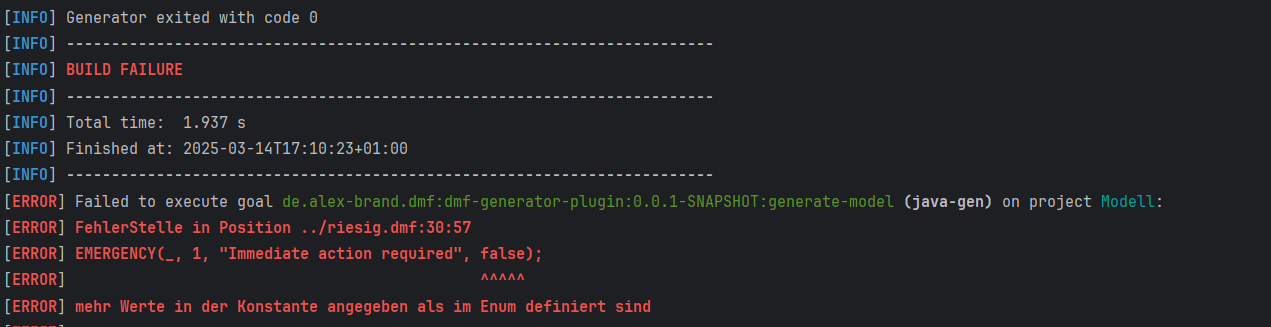
\includegraphics[width=\linewidth]{bilder/screenshot-error-generator}
        \caption{Ausgabe eines Fehlers}
        \label{fig:screenshot-error-generator}
    \end{figure}






\end{document}